\RequirePackage[ngerman=ngerman-x-latest]{hyphsubst}
\documentclass[ngerman]{tudscrreprt}
\usepackage[T1]{fontenc}
\usepackage{selinput}
\SelectInputMappings{adieresis={ä},germandbls={ß}}
\usepackage[defaultsans]{opensans}
\usepackage{babel}
\usepackage{hyperref}
\usepackage{graphicx}

\begin{document}
\faculty{Fakultät Informatik}
\institute{Institut für Systemarchitektur}
\chair{Professur für Datenschutz und Datensicherheit}
\date{01.07.2019}
\author{Lars Westermann, Jan Zimmermann, Alexander Römmer, Luzia Franke, Marvin Herrmann, Cornell Ziepel, Robert Ludwig, Bruno Bellmann, Adrian Gollmann, Jonas Dimitrow, Marcus Köhler, Paul Maximilian Pickhardt, Matthias Sebastian Theodor Schermuly, Moritz Pflügner, Andreas Geyer, Nico Volkens}
\title{Digitalisierung der Anrechnung von Studien- und Prüfungsleistungen}
\thesis{Seminararbeit}
\supervisor{Frau Dr.-Ing.Katrin Borcea-Pfitzmann}
\maketitle

\tableofcontents

\chapter{Einleitung}

\section{Motivation}

\section{Zielsetzung}

\section{Vorgehensweise}

\chapter{Analyse des herkömmlichen Prozesses/Verfahrens/Prozedur an der Fakultät Informatik der TU Dresden}

\section{Voraussetzungen für die Anrechnung von Studien - und Prüfungsleistungen (rechtliche Anforderungen)}

\section{Analyse und Bewertung der Teilprozesse und Stakeholder}

In diesem Kapitel werden die Stakeholder des neu zu entwickelnden Systems für die Anrechnung von Studien – und Prüfungsleistungen behandelt. Dabei wird auf deren Rolle im bisherigen Prozess eingegangen und die Veränderungen durch eine mögliche Einführung eines neuen Systems beschrieben. Das neue System hat vier Stakeholder: die Mitarbeiter des Prüfungsamtes, die Mitglieder des Prüfungsausschusses, die Studierenden und die zuständige IT-Abteilung.

\resizebox{\textwidth}{!}{%
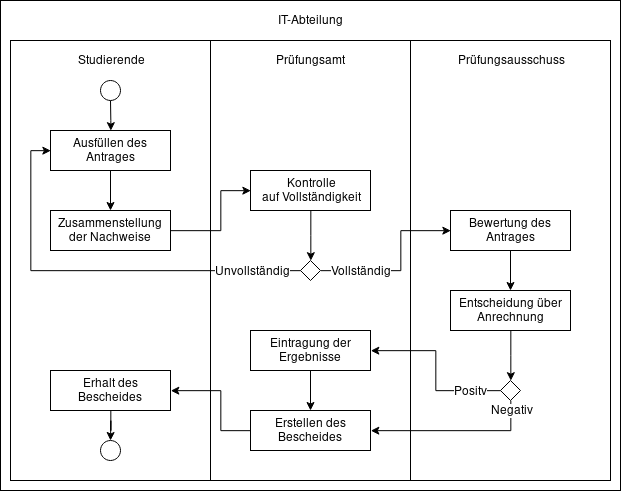
\includegraphics{images/analoger_prozess.png}%
}


\subsection{Prüfungsamt}

Im bisherigen Prozess nehmen die Mitarbeiter des Prüfungsamts die Anträge der Studierenden entgegen und bereiten die Dokumente für die Weitergabe an den Prüfungsausschuss vor. Nach der Überprüfung der Dokumente auf Vollständigkeit werden die Anträge an den Prüfungsausschuss weitergegeben. Wenn der Ausschuss seine Entscheidung über die Anrechnung getroffen hat, nimmt das Prüfungsamt das Ergebnis entgegen und trägt etwaige Noten in das Notenverwaltungssystem ein. Den Studierenden wird anschließend Bescheid über die Entscheidung des Ausschusses gegeben.

Durch die Einführung eines neuen Systems zur Einreichung und Bearbeitung der Anträge fällt das Prüfungsamt im Idealfall aus dem gesamten Prozess heraus. Die Entgegennahme und Aufbereitung der Anträge und Dokumente geschieht dann automatisiert und ohne den Einfluss des Prüfungsamtes. Das Eintragen der Ergebnisse bleibt möglicherweise Aufgabe das Amtes. Das hängt von der Automatisierbarkeit dieses Schrittes ab (TODO: rechtliches dazu klären).

\subsection{Prüfungsausschuss}

Momentan nehmen die Mitglieder des Prüfungsausschusses die zentrale Rolle in der Anrechnung von Studien – und Prüfungsleistungen ein. Der Prüfungsausschuss erhält die Anträge und Dokumente der Studierenden in aufbereiteter Form vom Prüfungsamt. Danach entscheidet der Ausschuss darüber, ob die Anrechnung ganz, teilweise oder gar nicht vorgenommen wird. Das Ergebnis der Entscheidung wird dann an das Prüfungsamt zurückgegeben.

Auch im neuen System würde der Prüfungsausschuss noch immer die Entscheidung über die Anrechnung treffen. Der Ablauf wäre aber einfacher und könnte schneller vollzogen werden. Die Rolle des Ausschusses ändert sich also nicht grundlegend, Entscheidungen könnten aber vereinfacht oder beschleunigt werden.

\subsection{Studierende}

Die Hauptaufgabe der Studierenden ist es die, für die Anrechnung nötigen, Dokumente zu sammeln. Dazu gehören beispielsweise eine Beschreibung der Module und die Nachweise über die erhaltenen Noten. Die Anträge können dann im Moment auf zwei Wegen erstellt werden. Entweder füllen die Studierenden die vom Prüfungsamt bereitgestellten PDF-Vorlagen von Hand oder mit einem entsprechenden PDF-Reader aus oder sie benutzen einen bereits existierenden Assistenten, welcher nach Eingabe der Daten die PDFs automatisch ausfüllt. Nach dem Ausfüllen müssen die Anträge beim Prüfungsamt persönlich abgegeben werden. Die Möglichkeit einer Einreichung per Mail oder Online gibt es momentan nicht. Nach dem Entscheidungsprozess erfahren die Studierenden das Ergebnis per Mail und finden die dazugehörigen Noten im Notenverwaltungssystem.

Durch das neue System würde sich der Prozess für die Studierenden entscheidend vereinfachen. Sie müssten dann zwar immer noch die Recherche und Sammlung der nötigen Dokumente übernehmen, können die Anträge aber komfortabler einreichen. Die Anträge könnten mit dem neuen System komplett online erstellt und eingereicht werden, ohne das die Studierenden zum Prüfungsamt gehen müssen. Nach dem Abschicken der Dokumente sollen die Studierenden eine verbindliche Bestätigung erhalten, die den Erfolg des Abschickens bescheinigt. Ähnlich wie bisher würden die Studierenden das Ergebnis der Entscheidung digital erhalten.

\subsection{IT-Abteilung}

Aktuell hat die IT-Abteilung fast keinen Kontakt zum Anrechnungsprozess, sie pflegt lediglich die Funktionalität des E-Mail Servers und des bisherigen Notenverwaltungssystems.

Mit dem neuen System würde für die IT-Abteilung ein weiterer Verantwortungsbereich hinzukommen. Es müsste die Funktionalität, Erreichbarkeit und Absicherung des neuen Systems gemäß den Anforderungen gewährleistet werden.

\section{Mögliche Auswirkungen auf die Stakeholder}

Veränderungen in etablierten Arbeitsprozessen können auf die Stakeholder signifikante Auswirkungen haben. Einige mögliche werden im folgenden Abschnitt analysiert.

Die Veränderungen können von den Mitarbeitern des Prüfungsamtes sowohl positiv als auch negativ aufgefasst werden. Positiv ist vor allem der Wegfall von Arbeit. Durch ein neues System könnte man das Prüfungsamt in diesem Bereich entlasten, sodass sich die Mitarbeiter stärker auf andere Aufgaben konzentrieren können. Das Prüfungsamt kann die Einführung dennoch negativ sehen. Das Verlieren von Verantwortlichkeit für bestimmte Prozesse wird häufig als schlecht empfunden. Außerdem kann die zunehmende Automatisierung Sorgen über die Zukunft der eigenen Arbeitsstelle erzeugen.

Für den Prüfungsausschuss ist diese Entwicklung deshalb vor allem positiv. Ein digitaler Prozess kann Zeit sparen, in der man sich vermehrt anderen Aufgaben zuwenden kann. Zusätzlich dazu würde für die Mitglieder vor allem der Komfort des Prozesses erhöht werden.

Im Endeffekt bietet das neue System für die Studierenden nur Vorteile. Der Komfort würde deutlich erhöht werden und es müsste sich nicht mehr Öffnungszeiten oder Ähnliches gehalten werden. Die Abgaben können problemlos mobil erledigt werden. Ansprechpartner gibt es für die Studierenden natürlich auch mit dem neuen System immer noch.

Das Hinzukommen von Verantwortlichkeiten kann negativ und positiv gesehen werden. Zum einen steigt natürlich der Arbeitsaufwand für die IT-Abteilung, zum anderen könnte dies durch zusätzliche Mitarbeiter gut ausgeglichen werden.

\chapter{Überführung in einen digitalen Prozess}

\section{Digitalisierbarkeit der Teilprozesse (welche Stakeholder entfallen, Prüfungsamt nötig?)}

\section{Evaluation und Adaption bestehender Umsetzungen}

\section{Fachliche Beschreibung eines eigenen Systems (evtl. Untergliederung)}

\section{Bewertung des digitalen Prozesses}

\chapter{Vergleich des analogen und digitalen Ansatzes}

\chapter{Datenschutzbetrachtung bezüglich der Pseudonymisierung}

\section{Existierende Verfahren}

\section{Einbindung in den digitalen Prozess}

\chapter{Zusammenfassung und Ausblick}

\end{document}